\chapter{Benutzeranleitung}

\section{Missionsliste}

\begin{figure}[H]
	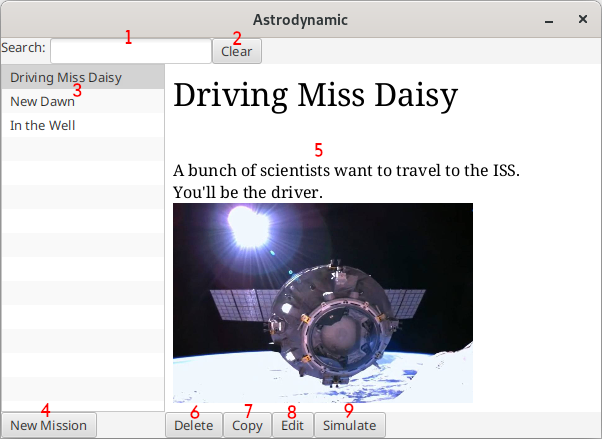
\includegraphics[width=12cm]{res/missionsliste.png}
	\caption{GUI Missionsliste mit Annotation}
\end{figure}

\begin{enumerate}
	\item Suchfeld
	\item Suchfeld leeren
	\item Liste verfügbarer Missionen
	\item Neue Mission öffnen im Missions-Editor
	\item Beschreibung der ausgewählten Mission
	\item Ausgewählte Mission löschen
	\item Ausgewählte Mission kopieren
	\item Ausgewählte Mission öffnen im Missions-Editor
	\item Ausgewählte Mission öffnen im Simulator
\end{enumerate}

\subsection{Grundlagen}
Die Missionsliste ist der Einstiegsbildschirm beim Start des Programs.
Hat der Benutzer keine Mission gespeichert welche geladen werden kann so werden drei Testmissionen geladen.
Am linken Rand befindet sich die Liste der verfügbaren Missionen.Anwählen einer Mission in der Liste per Klick mit der Linken Maustaste lädt die Missionsbeschreibung in den rechten Anzeigebereich und ermöglicht mit diese Mission per Buttons unten rechts am Bildschirmrand weiter zu Interagieren.

\subsection{Missionen nach Beschreibung suchen}
Das Suchfeld führt eine sofortige Textsuche auf Missions-Name und -Beschreibung durch und zeigt auf Basis dieser nur passende Missionen in der Liste der verfügbaren Missionen. Durch drücken des ''Suchfeld leeren''-Buttons können längere Sucheingaben sofort gelöscht und die Sortierung zurückgesetzt werden.

\subsection{Anlegen einer neuen Mission}
Klicken sie auf den ''Neue Mission öffnen im Missions-Editor''-Button unten links.
Es öffnet sich nun der Missions-Editor.
Für Details zum editieren einer Mission konsultieren sie das \hyperlink{missioneditor}{Kapitel Missions-Editor}.

\section{Simulator}

\hypertarget{missioneditor}{\section{Missions-Editor}}

\section{Planetoid-Editor}